% !TEX root = ../main.tex
%
\chapter{Methodology: Credal Semantic Entropy via Temperature Scaling}
\label{sec:methodology}
This chapter introduces a novel methodology that constructs a 
credal set for LLMs by dynamically scaling the decoding temperature.
By treating the temperature hyperparameter as a continuous parameter 
space and applying the statistical principles of relative likelihood,
we systematically filter out implausible distributions. We then 
extend semantic entropy to operate over this credal set, yielding
robust upper and lower uncertainty bounds that serve as a signal 
for hallucination detection.

\section{Overview of the Pipeline}
\label{sec:methodology:overview}
Our proposed methodology, which we term Credal Semantic Entopy,
works for a given input prompt $x$ (a question and optional context),
in four sequential stages:

\begin{enumerate}
    \item \textbf{Valid Temperature Selection (The $\alpha$-cut)}:
	Before generation, we must determine which temperatures
	produce statistically valid probability distributions. 
	Using a labeled dataset, we evaluate the model's 
	average Negative Log-Likelihood (NLL) as shown in 
	\ref{eq:average_nll}
	across a discrete grid of temperatures. 
	We identify the optimal temperature
	that minimizes the average NLL and compute the relative 
	likelihood for all temperatures. The $\alpha$-cut is 
	constructed by all temperatures with a relative likelihood
	greater or equal than $\alpha$.

    \item \textbf{Generation and Semantic Clustering}:
	Using the prompt $x$, the LLM generates multiple candidate
	responses at every valid temperature in the $\alpha$-cut.
	We cluster these generated sequences by their meaning
	over all valid temperatures. 

    \item \textbf{Computation of Cluster Probability Bounds}:
	For each valid temperature, we compute the probability
	of each semantic cluster. Because the temperature 
	modulates the entropy of the underlying token 
	distributions, the probability of a given cluster will 
	fluctuate across the $\alpha$-cut. By finding the 
	minimum and maximum probability assigned to each cluster 
	across all valid temperatures, we establish the lower 
	and upper bounds for every semantic concept.

    \item \textbf{Quantifying Epistemic Uncertainty}:
	Finally, we compute the Upper Shannon Entropy using these 
	bounds. This final scalar value is used to predict whether 
	the model is hallucinating.
\end{enumerate}

\begin{figure}
    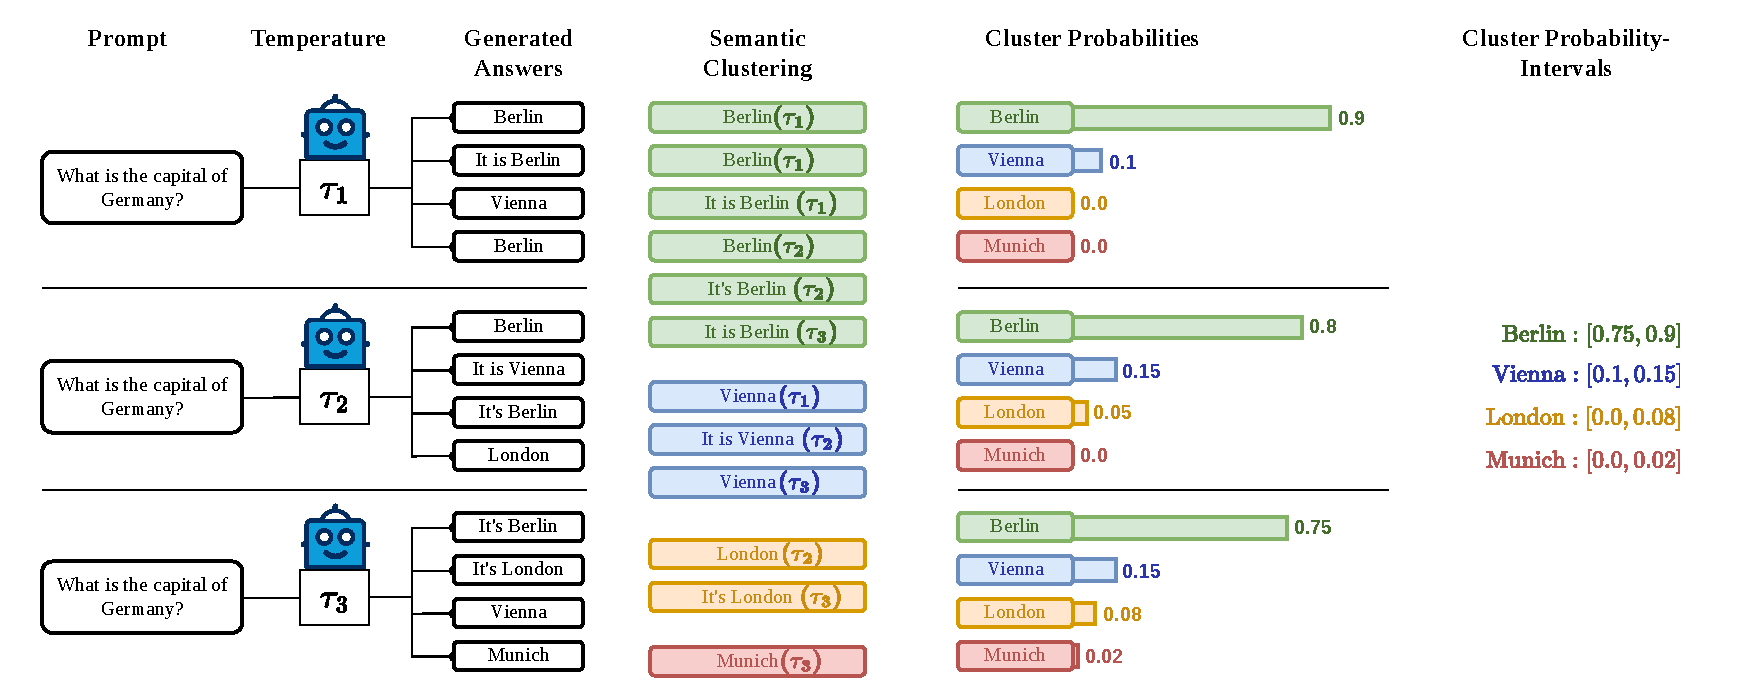
\includegraphics[width=\textwidth]{drawio/CredalSemanticEntropyClusterProbabilities.pdf}
    \caption{Visualization of the first three stages of our 
    methodology. The process 
    begins with multi-temperature generation, followed by semantic 
    clustering performed on the union of all generated sequences. 
    Finally, the probability mass of each cluster is marginalized at 
    every temperature to establish the robust probability intervals 
    used for uncertainty quantification.}
    \label{fig:methodology:pipeline_overview}
\end{figure}

The following sections formally define the mathematical and 
computational mechanics of each stage in this pipeline.




\section{Valid Temperature Selection (the $\alpha-$Cut)}
\label{sec:methodology:temperature_selection}
We consider the task of free-form Question Answering (QA) using a 
pre-trained, autoregressive LLM $\mathcal{M}$ with a vocabulary 
$\mathcal{V}$. This process is performed a priori using a labeled
training dataset or calibration dataset.
We evaluate a predefined grid of candidate temperatures $\mathcal{T}$.
For each temperature $\tau \in \mathcal{T}$, we measure its ability to
assign high probability to the ground-truth answers. This involves
three steps: computing the average NLL, deriving the relative 
likelihood and applying an $\alpha$-cut threshold.

\subsection{Computing the Average Negative Log-Likelihood}
\label{sec:methodology:temperature_selection:average_nll}
For every question-answer pair $(x^{(i)}, \mathbf{y}^{(i)})$ in the 
training dataset $\mathcal{D}_{\text{Train}}$ of size $D$, we compute the 
length-normalized NLL (\ref{eq:average_nll}) of the ground-truth answer 
sequence under the temperature-scaled probability distribution $P^{\tau}$.
The average NLL for a given temperature $\tau$ across the entire 
dataset is computed as: 

\begin{equation}
    \overline{\text{NLL}}(\tau) = 
	\frac{1}{D} \sum_{i=1}^{D} \left( - \frac{1}{T_i} 
	\sum_{t=1}^{T_i} \log P^\tau(y_t^{(i)} \mid 
	\mathbf{y}_{<t}^{(i)}, x^{(i)}) \right)
    \label{eq:temperature_nll}
\end{equation}

where $T_i$ is the length (number of tokens) of the $i$-th target 
sequence. This average NLL serves as our primary metric for evaluating
how well a specific temperature calibrates the model's output 
distribution to the true data distribution. We denote the optimal  
temperature that yields the minimum $\overline{\text{NLL}}$ as $\tau^{ML}$:

\begin{equation}
    \tau^{ML} = \argmin_{\tau \in \mathcal{T}} 
    \overline{\text{NLL}}(\tau)
    \label{eq:temperature_mle}
\end{equation}

\subsection{Deriving Relative Likelihoods}
\label{sec:methodology:temperature_selection:rel_likelihoods}
Because NLL values are absolute and can vary drastically depending
on the model and dataset, it is difficult to define a universal 
threshold for what constitutes a "good" temperature. To standardize
this, we map the average NLLs into the relative likelihood space.

As established in Equation \ref{eq:relative_likelihood},
the relative likelihood $\gamma(\tau)$ of any temperature is computed
by comparing its likelihood $L(\tau)$ to the optimal likelihood 
$L(\tau^{ML})$. In the logarithmic domain, this is equivalent to
to the exponentiated difference of their average NLLs:

\begin{equation}
    \gamma(\tau) = \displaystyle\frac{L(\tau)}{L(\tau^{ML})} 
	= \exp \left( - \left( \overline{\text{NLL}}(\tau) 
	- \overline{\text{NLL}}(\tau^{ML}) \right) \right)
    \label{eq:nll_relative_likelihood}
\end{equation}

By definition, the optimal temperature $\tau^{ML}$ has a relative likelihood
of $\gamma(\tau^{ML}) = 1.0$. All other temperatures $\tau$ will
have a relative likelihood $\gamma(\tau) \in [0,1]$, explicitly
quantifying how plausible they are compared to the best performing 
parameterization.

\subsection{The $\alpha$-Cut}
 \label{sec:methodology:temperature_selection:alpha_cut}
Following the framework of credal prediction 
\cite{löhr2025credalpredictionbasedrelative},
we apply an $\alpha$-cut, retaining only those temperatures whose
relative likelihood meets or exceeds a specified confidence 
threshold $\alpha \in [0,1]$.
The final set of valid temperatures is formally defined as:

\begin{equation}
    \mathcal{T}_\alpha = \{ \tau \in \mathcal{T} : 
    \gamma(\tau) \geq \alpha \}
    \label{eq:temperature_alpha_cut}
\end{equation}


\section{Generation and Semantic Clustering}
\label{sec:methodology:generation}
Once the set of valid temperatures $\mathcal{T}_\alpha$
has been established via the train dataset, we apply the methodology 
to the unseen test queries. For a given input prompt $x$, the goal is
to map the model's raw token outputs into discrete semantic concepts.
This requires a two-step process. Generating a diverse pool of 
candidate responses and clustering them based on semantic equivalence.

\subsection{Multi-Temperature Sequence Generation}
\label{sec:methodology:generation:sequence_generation}
The evaluate the model's uncertainty, we must sample responses from 
every valid temperature.
For each temperature $\tau \in \mathcal{T}_\alpha$, we prompt the 
LLM $\mathcal{M}$ to generate $N$ independent answer sequences.

Let $\mathcal{S}_\tau = \{ s_1^\tau, s_2^\tau, \dots, s_N^\tau \}$ 
denote the set of sequences generated at temperature $\tau$. The total
pool of generated responses for the prompt $x$ is the union of all 
sequences generated across all valid temperatures:

\begin{equation}
    \mathcal{S}_{total} = \bigcup_{\tau \in \mathcal{T}_\alpha} 
	\mathcal{S}_\tau
    \label{eq:pool_of_sequences}
\end{equation}

By generating across $\mathcal{T}_\alpha$, we force the model to 
explore different regions of its probability space. Lower temperatures 
favor the most likely tokens, whereas higher temperatures flatten the 
distribution, encouraging the model to output lower-probability claims.


\subsection{Bidirectional Entailment and Equivalence Classes}
\label{sec:methodology:generation:entailment}
As discussed in Section \ref{sec:related_work:semantic_entropy}, 
evaluating uncertainty on the raw lexical set $\mathcal{S}_{total}$ 
artificially inflates misconfidence due to the aleatoric linguistic 
variations. We therefore partition $\mathcal{S}_{total}$ into a set of 
semantic equivalence classes, or clusters, denoted as 
$C = \{ c_1, c_2, \dots, c_K \}$.

To determine if two distinct sequences $s_i$ and $s_j$ belong to the 
same cluster, we employ an automated Natural Language Inference (NLI)
model (e.g., DeBERTa-large-MNLI 
\cite{he2021debertadecodingenhancedbertdisentangled}).
The NLI model evaluates whether the premise sequence entails the 
hypothesis sequence. We define a strict semantic equivalence relation
$E(\cdot, \cdot)$ which holds true if and only if there is 
\textbf{bidirectional entailment}: 
$(s_i \models s_j) \land (s_j \models s_i)$

If $s_i$ entails $s_j$ and $s_j$ entails $s_i$, the sequences are 
deemed factually equivalent in the context of the prompt $x$ and are 
assigned to the same cluster $c_k$. Thus, a cluster holds all 
sequences  that belong to the same equivalence class of 
$E(\cdot, \cdot)$:  $\forall s, s' \in c_k : E(s, s')$. 
% NOTE: should I leave that in?

\subsection{Constructing the Cluster Probability Distributions}
\label{sec:methodology:generation:cluster_probability}
Once the clusters $C$ are established, we must compute the probability
of each cluster under each temperature $\tau \in \mathcal{T}_\alpha$.
The probability of a semantic cluster $c_k$ at temperature $\tau$ is 
the normalized sum of the likelihoods of all sequences within that 
cluster, evaluated under the distribution $P^\tau$:

\begin{equation}
    P^\tau(C_k \mid x) = 
    \frac{P^\tau(c_k \mid x)}{\sum_{c \in C} P^\tau(c \mid x)}
    \label{eq:normalized_credal_cluster_probs}
\end{equation}

where

\begin{equation}
    P^\tau(c_k \mid x) = \sum_{s \in c_k} P^\tau(s \mid x)
    \label{eq:credal_cluster_probs}
\end{equation}

This marginalization step is crucial. It abstracts away the specific
phrasing of the answers, yielding a set of discrete probability 
distributions $P^\tau(C)$ over the fundamental semantic meaning. 
It is important to note that the set of semantic clusters $C$
is global. It contains every unique meaning generated across 
\textit{all} valid temperatures.
If a specific cluster $c_k$ does not contain any sequences generated 
at a particular temperature $\tau$, we assign it a zero probabilty 
mass for that distribution. This ensures that every distribution 
$P^\tau$ is defined over the same common support $C$, allowing for 
the direct element-wise comparison required to compute the upper and
lower probability bounds in the next step. To compute the sequence
probability $P^\tau(s \mid x)$, we use the length normalized
NLL as defined in Equation \ref{eq:average_nll} because we do not want to
punish longer sequences 
\parencite{malinin2021uncertaintyestimationautoregressivestructured}. 
In the case where shorter answers are wanted, as it is in TriviaQA 
\parencite{joshi2017triviaqalargescaledistantly}, we could use the
unnormalized NLLs (\ref{eq:nll}) as well.

\subsection{Quantifying Credal Semantic Uncertainty}
\label{sec:methodology:uncertainty_quantification}
By scaling the temperature, we observe a range of probabilities for 
each semantic cluster. We utilize the observed probability 
fluctuations to establish upper and lower probability bounds for 
every semantic concept. The \textbf{credal set} is then formally
defined as the set of \textit{all} valid probability distributions 
that respect these element-wise bounds.

\textbf{Establishing Probability Bounds} \\
Let $C = \{ c_1, c_2, \dots, c_K \}$ be the set of identified semantic 
clusters. For each cluster $c_k$, we inspect its probability mass
across all valid temperatures $\tau \in \mathcal{T}_\alpha$
We define the \textbf{lower probability} $\underline{P}(c_k)$ and 
the \textbf{upper probability} $\overline{P}(c_k)$  as the minimum and 
maximum probabilities observed for that cluster. 

\begin{equation}
    \underline{P}(c_k) = \min_{\tau \in \mathcal{T}_\alpha} 
	P^\tau(c_k \mid x)
    \quad \quad
    \overline{P}(c_k) = \max_{\tau \in \mathcal{T}_\alpha}
	P^\tau(c_k \mid x)
    \label{eq:cluster_bounds}
\end{equation}

These bounds define an interval 
$[\underline{P}(c_k), \overline{P}(c_k)]$ representing the model's 
epistemic ambiguity regarding the plausibility of meaning $c_k$.

\begin{figure}
    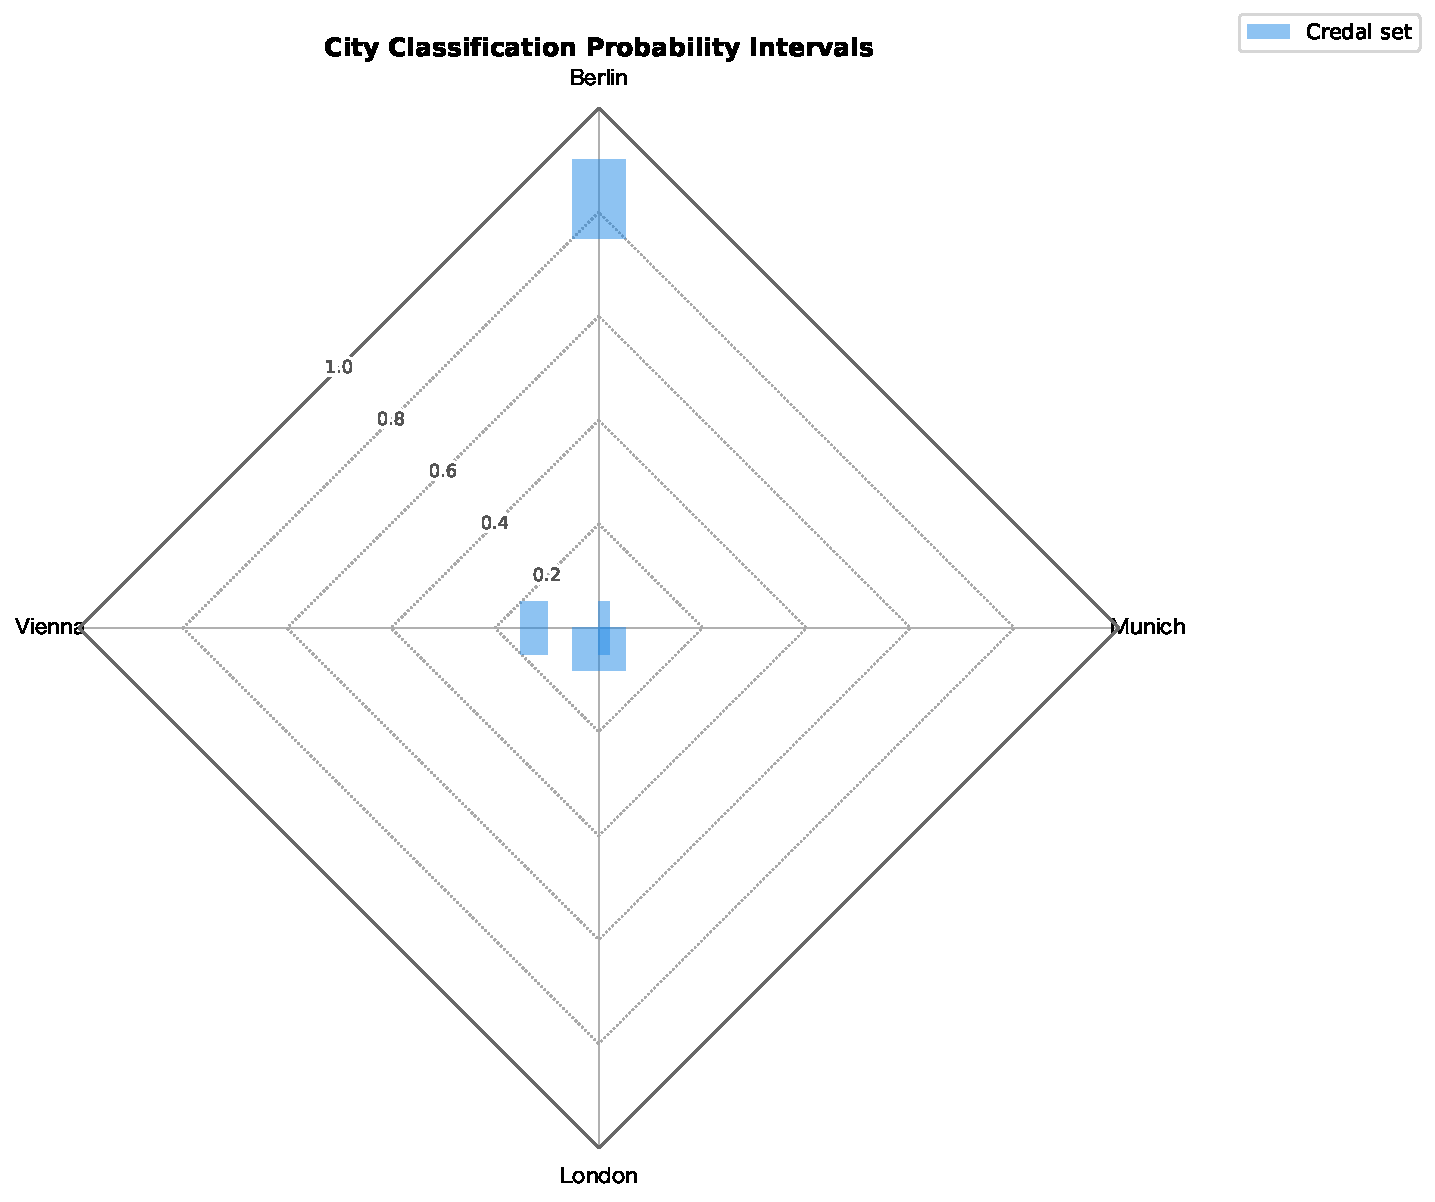
\includegraphics[width=0.7\textwidth]{gfx/city_classification_intervals.pdf}
    \caption{Geometric representation of the credal set derived from the 
    probability intervals established in Figure 
    \ref{fig:methodology:pipeline_overview}. Each axis of the radar chart 
    corresponds to a distinct semantic cluster. The blue bars represent the
    probability intervals (lower to upper bounds) for each class, 
    illustrating the model's epistemic uncertainty across the potential 
    predictions. This visualization approach follows [Hof+26].}
    \label{fig:methodology:visual_probability_bounds}
\end{figure}

\textbf{Defining the Credal Set} \\
We construct the credal set $\mathcal{K}$ as the convex set of all 
probability distributions $P$ over $C$ that are consistent with these
interval bounds. Formally:

\begin{equation}
    \mathcal{K} = \left\{ P \in \Delta_K \mid \forall k: 
	\underline{P}(c_k) \leq P(c_k) \leq \overline{P}(c_k),
	\sum_{k = 1}^K P(c_k) = 1 \right\}
    \label{eq:credal_set}
\end{equation}

where $\Delta_K$ denotes the standard probability simplex. By defining
$\mathcal{K}$ via these bounds, we capture not just the specific 
distributions observed at sampled temperatures, but the entire region 
of probability space supported by the valid relative likelihoods.

\textbf{Upper Semantic Entropy ($H^*$)} \\
This metric corresponds to the maximum entropy (highest uncertainty)
attainable by any distribution within the credal set. It serves as 
our primary signal for hallucination detection 
(\ref{sec:background:credal_sets:uncertainty}), 
identifying cases 
where the model's interval constraints allow for a highly flat, 
uniform distribution:

\begin{equation}
    H^*(x) = \max_{P \in \mathcal{K}} 
	\left( - \sum_{k=1}^K P(c_k) \log P(c_k) \right)
    \label{eq:upper_semantic_entropy}
\end{equation}

\textbf{Lower Semantic Entropy ($H_*$)} \\
Conversely, the lower entropy corresponds to the most deterministic
distribution consistent with the bounds: 

\begin{equation}
    H_*(x) = \min_{P \in \mathcal{K}}
	\left( - \sum_{k=1}^K P(c_k) \log P(c_k)\right)
    \label{eq:lower_semantic_entropy}
\end{equation}

The difference $H^* - H_*$ reflects the magnitude of epistemic 
uncertainty as shown in Section
\ref{sec:background:credal_sets:uncertainty}. 
For the experimental evaluation in this thesis, we utilize the 
upper semantic entropy $H^*$, as it provides the most conservative 
safety guarantee by considering the maximum plausible uncertainty.

